\documentclass{article}



\usepackage{arxiv_parts/arxiv}

\usepackage{amsmath,amssymb,amsfonts}
\usepackage{algorithmic}
%\usepackage{breqn}
\usepackage{graphicx}
\usepackage{caption}
\usepackage{subcaption}
\usepackage{textcomp}
\usepackage{xcolor}
\usepackage{amsthm}
\usepackage{enumerate}
%\usepackage{multicol}
%\usepackage{blindtext, subfig}
%\usepackage{dblfloatfix} % fix for bottom-placement of figure
%\usepackage{natbib}
\usepackage{dsfont}
\usepackage{siunitx}
%multi-row
\usepackage{multirow}
\usepackage{bbm}
\usepackage{bm}
\makeatletter
\newcommand{\Spvek}[2][r]{%
  \gdef\@VORNE{1}
  \left(\hskip-\arraycolsep%
    \begin{array}{#1}\vekSp@lten{#2}\end{array}%
  \hskip-\arraycolsep\right)}

\def\vekSp@lten#1{\xvekSp@lten#1;vekL@stLine;}
\def\vekL@stLine{vekL@stLine}
\def\xvekSp@lten#1;{\def\temp{#1}%
  \ifx\temp\vekL@stLine
  \else
    \ifnum\@VORNE=1\gdef\@VORNE{0}
    \else\@arraycr\fi%
    #1%
    \expandafter\xvekSp@lten
  \fi}
\makeatother


 
\newtheorem{Theorem}{Theorem}
\newtheorem{Proposition}{Proposition}

\newcommand{\W}{\mathcal{W}}
%\newcommand{\Deellip}{\textit{DEEL.LIP}\footnote{https://github.com/deel-ai/deel-lip to be %published soon}
%}
\newcommand{\Deellip}{\textit{DEEL.LIP}\footnote{https://github.com/deel-ai/deel-lip}}
\renewcommand{\arraystretch}{1.3}
\setlength{\tabcolsep}{4pt}
\usepackage[pagebackref=true,breaklinks=true,colorlinks,bookmarks=false]{hyperref}

\begin{document}

%\title{hinge regularized optimal transportation for robust classification}
\title{Achieving robustness in classification using optimal transport with hinge regularization}
\author{%
  Mathieu Serrurier\\
  IRIT\\
  Université Paul Sabatier Toulouse
  \And
  Franck Mamalet\\
  IRT Saint-Exupery
  \And
  Alberto González-Sanz\\
  IMT\\
  Université Paul Sabatier Toulouse
  \And
  Thibaut Boissin\\
  IRT Saint-Exupery
  \And
  Jean-Michel Loubes \\
  IMT\\
  Université Paul Sabatier Toulouse
  \And
  Eustasio del Barrio \\
  Dpto. de Estadística e Investigación Operativa\\
  Universidad de Valladolid
  
}
\maketitle
\begin{abstract}
%It has been shown that constraining the Lipschitz constant of a deep neural networks increases the robustness against adversarial attacks. We propose a new framework of binary classification based on optimal transport that integrates these structural constraint as a theoretical requirement. We propose to compute networks that are the solution of an hinge regularized version of the Kantorovich-Rubinstein dual formulation for the estimation of the Wasserstein distance. The loss function obtained has a direct interpretation in terms of adversarial robustness together with certifiable robustness bound. We prove that this classification formulation has a solution, and is still the dual formulation of an optimal transportation problem despite the use of the hinge regularization. We also establish the geometrical properties of this optimal solution and we extend the approach to multi-class problems. The experiments show that the approach provides the expected guarantees in terms of robustness without any significant accuracy drop. The results also suggest that adversarial attacks on the proposed models visibly and meaningfully change the input, and can thus serve as an explanation for the classification.

Adversarial examples have pointed out Deep Neural Networks vulnerability to small local noise. It has been shown that constraining their Lipschitz constant should enhance robustness, but make them harder to learn with classical loss functions. We propose a new framework for binary classification, based on optimal transport, which integrates this Lipschitz constraint as a theoretical requirement. We propose to learn 1-Lipschitz networks using a new loss that is an hinge regularized version of the Kantorovich-Rubinstein dual formulation for the Wasserstein distance estimation. This loss function has a direct interpretation in terms of adversarial robustness together with certifiable robustness bound. We also prove that this hinge regularized version is still the dual formulation of an optimal transportation problem, and has a solution. We also establish several geometrical properties of this optimal solution, and extend the approach to multi-class problems. Experiments show that the proposed approach provides the expected guarantees in terms of robustness without any significant accuracy drop. The adversarial examples, on the proposed models, visibly and meaningfully change the input providing an explanation for the classification.



% We also experimented adversarial attack on the proposed model, which suggests that visible and meaningfull changes must be made to the input in order to be mis-classified. This opens perspectives to 
%The results also suggest that adversarial attacks on the proposed models require to perform explicit change on the input critical part, and can thus serve as an explanation for the classification.



\end{abstract}


% keywords can be removed
%\keywords{First keyword \and Second keyword \and More}
\section{Introduction}
\label{sec:intro}
The important progress in deep learning has led to a massive interest for these approaches in industry. However, when applying machine learning to critical tasks such has in the transportation or the medical domain, empirical and theoretical guarantees are required. Unfortunately, it has been shown that neural networks are weak to adversarial attacks: a carefully chosen small shift to the input, usually indistinguishable from noise, can change the class prediction \cite{szegedy2013}.  This sensitivity to adversarial attacks is mainly due to the Lipschitz constant of a neural network which can be arbitrarily high when unconstrained. Most of white-box attacks (where the full model is available) take advantage of it to build adversarial examples by using gradient descent with respect to the input variables. $FGSM$~\cite{Goodfellow2014a} performs only one step of gradient descent when other approaches such as $PGD$~\cite{Madry2017,carlini2017towards} find the optimal adversarial example iteratively. In black-box scenarios, gradients or logits of the model are not available. In such case, attacks start from large perturbations and then reducing it step by step (see for instance, boundary attacks~\cite{Brendel2018} and pointwise attacks~\cite{Schott2018}).

There are three major types of strategy to address the issue of adversarial attacks. Agnostic defenses are independent of the model and consist in altering the input or the prediction. For instance, Cohen et al. obtain a provable certificate with respect to $l_2$ norm by using Gaussian random smoothing~\cite{pmlr-v97-cohen19c}. DEFENSE-GAN~\cite{samangouei2018defensegan} uses a GAN to transform the input into the closest non-adversarial one at inference time. The second group of strategies relies on saddle point optimization by adding a penalty term measuring the empirical weakness against adversarial example during the learning process~\cite{Madry2017}. The last type of approaches focus on the Lipschitz constant of the network. It has been proven that bounding the  Lipschitz constant of a neural network provides certifiable robustness guarantees against local adversarial attacks~\cite{hein_formal_2017,ono_lightweight_2018}, improves generalizations~\cite{Sokolic_2017} and the interpretability of the model~\cite{tsipras2018robustness}.  This constraint can be achieved layer by layer by using spectral normalization~\cite{cisse_parseval_2017} or non-expansive layer~\cite{qian_l2-nonexpansive_2019}. In \cite{li2019preventing}, Li et al. go beyond the Lipschitz constant bounding by requiring layers to be gradient norm preserving. Combined with hinge loss, it allows them to achieve stronger robustness certification. However, the main limitation of this approach relies in the link between the hinge margin parameter and the robustness of the network.

In this paper we propose a new classification framework based on optimal transport that integrates the Lipschitz constant and the gradient norm preserving constraint as a theoretical requirement. To the best of our knowledge, very few researches investigate the link between binary classification and optimal transport (in~\cite{Frogner2015}, Frogner et al. use Wasserstein loss to improve multilabel classification). In Wasserstein GAN~\cite{Arjovsky2017}, the k-Lipschitz networks used to measure the distance between two distributions act like a discriminator, in analogy with the initial GAN algorithm \cite{Goodfellow2014}. The Wasserstein distance is approximated using a loss based on the Kantorovich-Rubinstein dual formulation and a k-Lipschitz network constrained by weight clipping. However, as we will demonstrate, a vanilla classifier based on the Kantorovich-Rubinstein loss is suboptimal, even on toy datasets.

We propose a binary classifier based on a regularized version of Kantorovich-Rubinstein formulation using a hinge loss term. We show that it remains the dual of an optimal transport problem, and we prove that the optimal solution of the problem exists and makes no error when the classes are well separated. With this new optimization problem, we guarantee to have an accurate classifier with a loss that is defined on and takes advantage of 1-Lipschitz function. As in~\cite{li2019preventing}, we bound the Lipschitz constant of the linear layers by B\"jorck normalization and use norm preserving activation functions~\cite{pmlr-v97-anil19a}. However, the optimal transport interpretation of the problem makes the bridge between these constraints and the loss function. When solving this optimal transport problem, attacking a prediction corresponds to travel along the transport plan up to the decision frontier. The output of the optimal network is linked to the length of this path, which is maximized during the optimization process of the proposed loss. 

The paper, and the contributions, are structured as follows. In Section~\ref{sec:wass_distance}, we recall the definition of Wasserstein distance and the dual optimization problem associated. We present the interesting properties of a classifier based on this approach, illustrate that it leads to a suboptimal classifier even on a toy dataset. Section~\ref{sec:kr_hinge} describes the proposed binary classifier, based on a regularized version of the Kantorovich-Rubinstein loss with a hinge regularization. We show that the primal of this classification problem is a new optimal transport problem and we demonstrate different mathematical properties of our approach. Section~\ref{sec:lip_const} is devoted to the way of constraining the classifier to be  1-Lipschitz and how to generalize the approach to multi classification problems. Section~\ref{sec:experimentation} presents the results of  experiments on MNIST, Cifar10 and CelebA datasets, measuring and comparing the results of different approaches in terms of accuracy and robustness. Last, we demonstrate that with our approach, building an adversarial example requires explicitly changing the example to an in-between two-classes image, which correspond to a point halfway on the transport plan. Proofs, computations details and additional experiments are reported in the appendix. 



\section{Wasserstein distance and Kantorovich-Rubinstein classifier}
\label{sec:wass_distance}
\input{arxiv_parts/wass_distance_arxiv}


\section{Hinge regularized Kantorovich-Rubinstein classifier }
\label{sec:kr_hinge}
\input{arxiv_parts/hkr_arxiv}

\section{Architecture}
\label{sec:lip_const}
\subsection{1-Lipschitz gradient norm preserving network}
In order to build a deep learning classifier based on the hinge-KR optimization problem (Eq.~\eqref{eq:reg_OT}), we have to constrain the Lipschitz constant of the neural network to be equal to 1.  It is known that evaluating it exactly is a NP-hard problem~\cite{NIPS2018_7640}. The simplest way to constraint a network to be 1-Lipschitz is to impose this 1-Lipschitz property to each layer. For dense layers, the initial version of WGAN \cite{Arjovsky2017} consisted of clipping the weights of the layers. However, this is a very crude way to upper-bound Lipschitz constant. Normalizing by the Frobenius norm has also been proposed in~\cite{SalimansK16}. In this paper, we use spectral normalization as proposed in~\cite{Miyato2018SpectralNF}, since the spectral norm is equals to the Lipschitz constant of the layer. At the inference step, we normalize the weights of each layer by the spectral norm of the matrix. This spectral norm is computed by iteratively evaluating the largest singular value with the power iteration algorithm~\cite{GOLUB200035}. This is done during the forward step and taken into account for the gradient computation. In the case of 2D-convolutional layers, normalizing by the spectral norm of convolution kernels is not enough and a supplementary multiplicative constant $\Lambda$ is required (the regularization is then done by dividing $W$ by $\Lambda||W||$). We propose, for zero padding, a tighter estimation of $\Lambda$ than the one proposed in~\cite{cisse_parseval_2017}, computing the average duplication factor of non zero padded values in the feature map:

\begin{equation}
\Lambda=\sqrt{\frac{(k.w-\bar{k}.(\bar{k}+1)).(k.h-\bar{k}.(\bar{k}+1))}{h.w}}
\label{eq:ConvApproxLip}
\end{equation}
for a kernel size equals to $k=2*\bar{k}+1$.
Even if this constant doesn't provide a strict upper bound of the Lipschitz constant (for instance, when the higher values are located in the center of the picture), it behaves very well empirically.
Convolution with stride, pooling layers, detailed explanations and demonstrations are discussed in Appendix~\ref{sec:convStride}.\\

As shown in Property~\ref{coro_norm1}, the optimal function $f^*$ with respect to Eq.~\eqref{eq:reg_OT}, verifies $||\nabla f^* ||=1$ almost surely (\textit{gradient norm preserving} (GNP) architecture~\cite{pmlr-v97-anil19a} ). We apply the approach described in~\cite{pmlr-v97-anil19a}, based on the use of specific activation functions and a process of normalization  of the weights. Two norm preserving activation functions are proposed: i)\ \textbf{GroupSort2} : sorting the vector by pairs, ii) \textbf{FullSort} : sorting the full vector.
These functions are vector-wise rather than element-wise. We also use the P-norm pooling~\cite{boureau2010}, with $P=2$ which is a norm-preserving average pooling.
Concerning linear functions, a weight matrix $W$ is gradient norm preserving if and only if all the singular values of $W$ are equals to $1$. In \cite{pmlr-v97-anil19a}, the authors propose to use the Björck orthonormalization algorithm \cite{bjorck71Ortho}. This algorithm is fully differential and, as for spectral normalization, is applied during the forward inference, and taken into account for back-propagation (see Appendix~\ref{app:normpreserving} for details). We don't consider BCOP \cite{qian_l2-nonexpansive_2019}, which performs slightly better that Björck for convolution but at an higher computation cost. We developed a full tensorflow~\cite{tensorflow2015-whitepaper} implementation in an opensource library, called \Deellip, that enables training of $k$-Lipschitz neural networks, and exporting them as standard layers for inference. 
\subsection{Multi-class hinge-KR classifier}
To adapt our approach to the multi-class case, we propose to use $q$ binary one-vs-all classifiers, where $q$ is the number of classes. The set of labels is now $Y=\{C_1,\ldots,C_q\}$. We name $P_k=\mathbb{P}(X|Y= C_k)$ and $\neg P_k=\mathbb{P}(X|Y\not = C_k)$ the  conditional  distributions  with  respect  to  $Y$. We obtain the following optimization problem :
\begin{equation}
\label{eq:hkr_multi}
\begin{split}
&\underset{f_1,\ldots,f_q \in Lip_1(\Omega)}{\text{sup}}-\mathcal{L}^{hKR}_\lambda(f_1,\ldots,f_q) \\
&\text{where}\\
&\mathcal{L}^{hKR}_\lambda(f_1,\ldots,f_q) = \sum_{k=1}^q \left[\underset{\textbf{x}  \sim \neg P_k}{\mathbb{E}} \left[f_k(\textbf{x})\right] -\underset{\textbf{x} \sim P_k}{\mathbb{E}}\left[f_k(\textbf{x})\right]   +\lambda\underset{\textbf{x}}{\mathbb{E}} \left(m-(2*\underset{y=C_k}{\mathbbm{1}} -1).f_k(x)  \right)_+ \right].
\end{split}
\end{equation}
The global architecture is the same as the binary one except that the last layer has $q$ outputs. For this last layer, each weights corresponding to each output neuron are normalized independently creating $q$ 1-Lipschitz functions with gradient norm preserving properties. With this architecture, the optimal transport interpretation is still valid. The class predicted corresponds to the argmax of the classifier functions. With this approach, the provable robustness lower-bound is the half of the difference between the max and the second max values of $\{f_1(x),\ldots,f_q(x)\}$.  

In \cite{li2019preventing}, Li et al. use classical multi-class hinge loss based on un-centered margin and apply constraint on the entire last layers rather than doing it independently. It allows to a lower provable adversarial robustness bound than ours. However, the $f_1,\ldots,f_q$ obtain in this setting are no more 1-Lipschitz one by one, making the adversarial robustness bounds not comparable directly (see Appendix~\ref{sec:robustness_bounds}).

\section{Experiments}
\label{sec:experimentation}
\begin{figure*}
\centering
\begin{subfigure}{.24\textwidth}
  \centering
  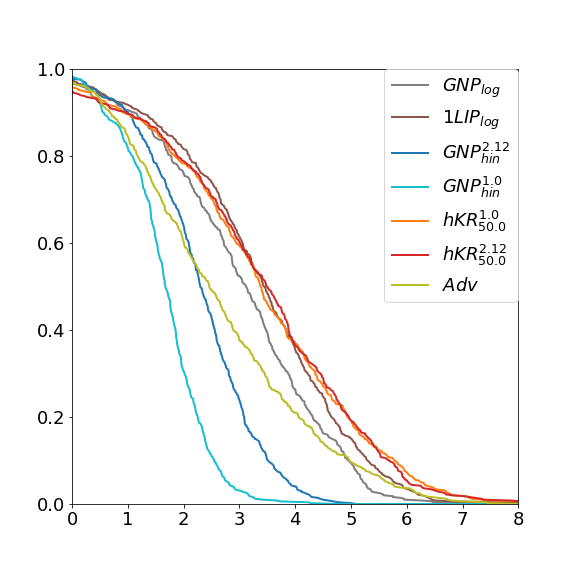
\includegraphics[width=1\linewidth]{cvpr_img/mnist_dense_adv_noise_norm_L2DeepFoolAttack.png}
  \caption{MNIST dense}
  \label{fig:l2norm_MLP_wass}
\end{subfigure}%
\begin{subfigure}{.24\textwidth}
  \centering
  
\includegraphics[width=1\linewidth]{cvpr_img/mnist_smallconfig_adv_noise_norm_L2DeepFoolAttack.png}
  \caption{MNIST CNN}
  \label{fig:l2_norm_VGG_wass}
\end{subfigure}
\begin{subfigure}{.24\textwidth}
  \centering
  
\includegraphics[width=1\linewidth]{cvpr_img/cifar10_verylarge_adv_noise_norm_L2DeepFoolAttack.png}
  \caption{CIFAR}
  \label{fig:l2_norm_MLP_lipsigmoid}
\end{subfigure}
\begin{subfigure}{.24\textwidth}
  \centering
  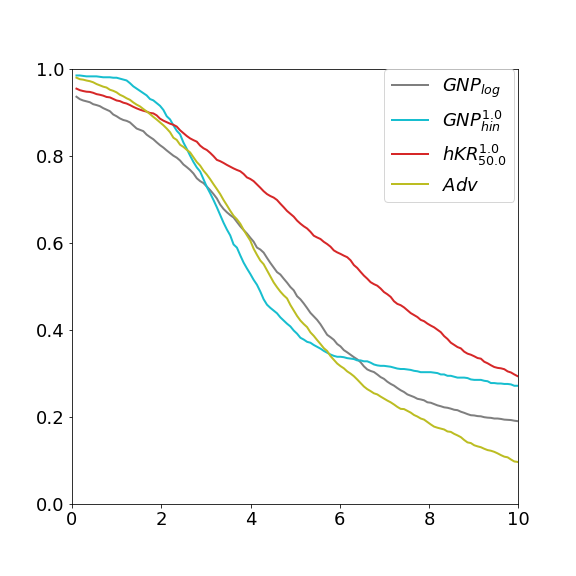
\includegraphics[width=1\linewidth]{cvpr_img/celeb_a_deepfool.png}
  \caption{CelebA}
  \label{fig:l2_norm_MLP_lipsigmoid}
\end{subfigure}
\caption{Accuracy (Y-axis) w.r.t. of $l_2$ norm of fooling noise with deepfool attack (X-axis) on 2000 images of the test set
}
\label{fig:deepfool_curves}
\end{figure*}

In the experiment, we compare five approaches: i) $Adv$ for Adversarial learning as in~\cite{Madry2017} , ii) $1LIP_{log}$ for log-entropy classifier with Björck orthonormalization and ReLU activation functions similar to Parseval networks~\cite{cisse_parseval_2017}, iii) $GNP^m_{hin}$ for gradient norm preserving classifiers based on hinge loss with margin $m$ as done in~\cite{li2019preventing} iv) $GNP_{log}$ for gradient norm preserving classifiers based on log entropy loss and v) $hKR^m_\alpha$ for gradient norm preserving classifiers based on the proposed hinge-KR with margin $m$ and coefficient $\alpha$. Note that, to the best of our knowledge, the $GNP_{log}$ hasn't been applied yet for adversarial defenses. To have a fair comparison, all the classifiers share the same dense or convolutional architectures except for the weight normalization and the activation functions. We set $\alpha$ to $50$ and margin $m$ to $1$ except for MNIST where we also consider $m=2.12$ to be comparable with the experiments in~\cite{li2019preventing}. For the $GNP$ classifiers, we apply Björck orthonormalization (15 steps with p=1) after the spectral normalization (this improves the convergence of the Björck algorithm). We use fullsort activation function for dense layers, and GroupSort2 for the convolutional ones.  Appendix~\ref{sec:networks_architecture} provides the full description of the architecture and the optimization process.

We consider three classification problems, two multi-class problems (MNIST~\cite{lecun-mnisthandwrittendigit-2010} and CIFAR-10~\cite{Krizhevsky09learningmultiple}) and a binary one (eyeglasses detection in Celeba-A dataset \cite{liu2015faceattributes}). For MNIST and CIFAR-10, we use standard configurations with 10 classes and no data augmentation, $50 000$ examples in the training set and $10 000$ examples in the test set. In the binary problem, we consider the separation between people with or without eyeglasses on the CelebA dataset with 128x128x3 centered images. This is an unbalanced classification problem with $16914$ examples in the training set ($38\%$ with eyeglasses) and $16914$ examples in the test set ($38\%$ with eyeglasses).

Figure \ref{fig:deepfool_curves} presents the robustness against $l_2$ attacks with \textit{DeepFool} attack~\cite{moosavi-deepfool15} on the different datasets. We use this type of attack since none of the tested approaches is specifically built to resist to it. We can observe that the $hKR^m_\alpha$ approach is at the top of robustness on all the dataset and systematically better than $GNP_{log}$ on all datasets and $GNP^m_{hin}$ on the multiclass problem for the same value of $m$. On the CelebA dataset, $GNP^m_{hin}$ and the adversarial approach $Adv$ start with a better accuracy, but don't resist to large attacks. $GNP_{log}$ and $1LIP$ have good performances on MNIST and CIFAR but their performances decrease when the models are deeper as for CelebA dataset ($1LIP$ was unable to converge on CelebA). To compare the different defense methods, we also apply a combination of the state-of-the art attacks $FGSM$~\cite{Goodfellow2014a}, $PGD$~($l_2PGD$) \cite{Madry2017} and  Carlini and Wagner ($l_2CW$) \cite{carlini2017towards} on 500 images of the test set. All attacks are performed with the  foolbox library~\cite{rauber2017foolbox}. For each value of $\epsilon$, we run all the attacks and consider it as a success if at least one of them has succeeded. The results are presented in Figure~\ref{fig:combine_curves} and Table~\ref{tab:celeba_comparison} details the robustness values for CelebA. The results confirm and amplify the ones obtained with deepfool attacks. $hKR^m_\alpha$ obtain the highest level of robustness in all the situations for low and high values of $\epsilon$. 
$Adv$ has the highest robustness w.r.t. $FGSM$ attacks, since it was designed against to, but is a bit less resistant w.r.t. $l_2PGD$ and weak w.r.t. $l_2CW$. $hKR^m_\alpha$ is especially strong w.r.t. Carlini and Wagner attack even with high values of $\epsilon$. The discrepancy between the robustness of the approaches increase when models become deeper. On the CelebA dataset,  $GNP_{log}$ have difficulties to resist to higher noise. As expected, $hKR^m_\alpha$ seems to take most advantage of the gradient norm preserving architecture and obtains robustness against large attacks with an acceptable decrease of accuracy without noise. 

Moreover, Table \ref{tab:celeba_comparison} shows that, for the proposed solution, accuracies w.r.t. $\epsilon$ are similar regardless the attacks. This suggests that optimal attacks are the same, and they are in the direction of the gradient of the classifier. This confirms the intuition pointed out in section~\ref{sec:khr_properties} that optimal attack consists on traveling along the optimal transport map. In Figure~\ref{fig:Deep_fool_CelebA}, we compare adversarial images obtained with $l_2$ deepfool for the different models. The first row corresponds to the initial image. The following rows except the last one, are pictures obtained after attacks for the different models. We design the attacks to push the image just beyond the classification boundary (50/50).  For the Madry et al. approach ($Adv$) the noise is barely detectable. The noise is more visible with the gradient preserving approaches $GNP_{log}$ and $GNP^m_{hin}$ but it is still hard to interpret and sometimes meaningless. In contrast to the other approaches, the noise required to change the output class for the $hKR$ classifier is highly structured, and interpretable. For people without glasses, the attack adds noise around the eyes and at the top of the nose. For people with eyeglasses, the attack tends to erase the glasses around the eyes and at the top of the nose. 

The last row corresponds to the scheme proposed in Section~\ref{sec:khr_properties} $att(\hat{f},\textbf{x})\approx x-2*\hat{f}(\textbf{x})*\nabla_x \hat{f}(\textbf{x})$ where $\hat{f}$ is the $hKR^1_{50}$ model. Indeed, if $\nabla_x \hat{f}(\textbf{x})=1$ and $\hat{f}(\textbf{x})$ is the distance between the $\textbf{x}$ and its image with respect to the transport, we expect to have $att(\hat{f},\textbf{x})=tr(\hat{f},\textbf{x})$. The  shifts are similar to the attacks and even more meaningful. This confirms that attacks against $hKR$ can be interpreted as a transportation from a class to the other one and then requires to explicitly change the transport image in the opposite class. This suggests that attacks can explain classification for the $hKR$ model. Moreover, the gradient of this model allows to build this explanation without relying on time-consuming algorithms.  



\begin{figure*}
\centering
\begin{subfigure}{.24\textwidth}
  \centering
  
\includegraphics[width=1\linewidth]{cvpr_img/mnist_dense__minAccuracy_L2attacks.png}
  \caption{MNIST dense}
\end{subfigure}%
\begin{subfigure}{.24\textwidth}
  \centering
  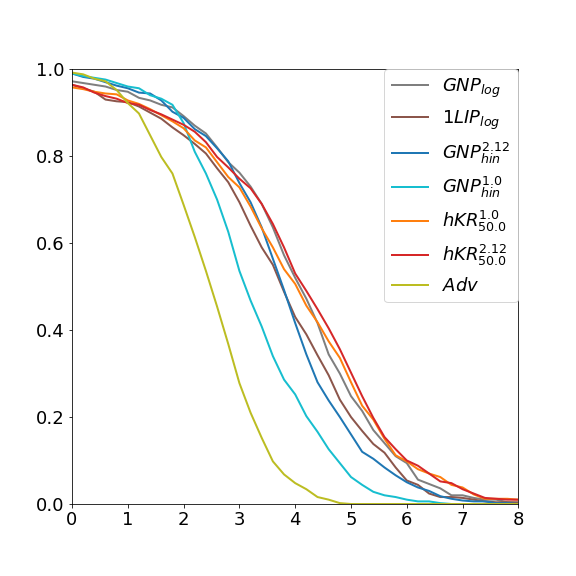
\includegraphics[width=1\linewidth]{cvpr_img/mnist_smallconfig__minAccuracy_L2attacks.png}
  \caption{MNIST CNN}
\end{subfigure}
\begin{subfigure}{.24\textwidth}
  \centering
  
\includegraphics[width=1\linewidth]{cvpr_img/cifar10_verylarge__minAccuracy_L2attacks.png}
  \caption{CIFAR}
\end{subfigure}
\begin{subfigure}{.24\textwidth}
  \centering
  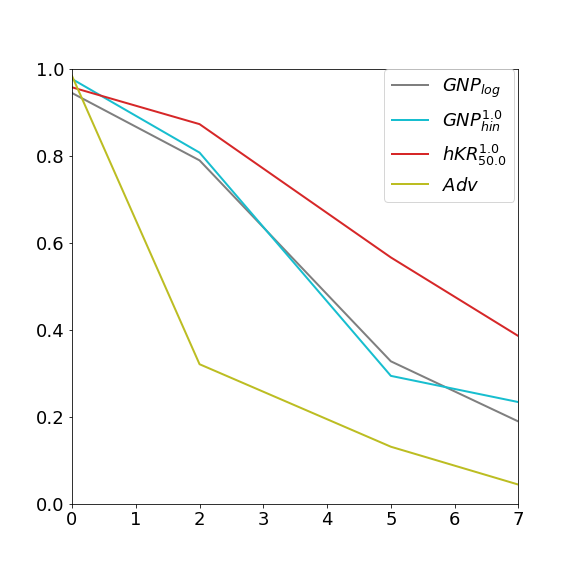
\includegraphics[width=1\linewidth]{cvpr_img/celeb_a_deepfool_all.png}
  \caption{CelebA}
\end{subfigure}
\caption{Accuracy (Y-axis) w.r.t. of $l_2$ norm of $FGSM$, $l_2PGD$, deepfool and $l_2$ Carlini and Wagner combined attacks on 500 images of the test set
}
\label{fig:combine_curves}
\end{figure*}



\begin{table}[]
    \centering

\begin{tabular}{|c|c|c|c|c|c|}
\hline
                          & $\epsilon$   & $Adv$ & $GNP_{hin}$ & $GNP_{log}$ & $hKR_{50}$\\ \hline
Base                      &   0   &   \textbf{98.04 }  &  97.2        &       94.51    &     96.07         \\ \hline
\multirow{2}{*}{$FGSM$} & $2$     &    \textbf{90.52 } &   86.79      &         81.40  &    87.44             \\ \cline{2-6} 
                          &  $5$  &  \textbf{ 82.96  } &     37.70    &      43.90     &     64.01                \\ \hline
\multirow{2}{*}{$l_2 GPD$}&  $2$            & 81.98    &     88.65    &    84.17       &\textbf{88.75  }           \\ \cline{2-6} 
                          &    $5$      &   61.35      &    34.90     &    48.02       &              \textbf{69.79  }     \\ \hline
\multirow{2}{*}{$l_2 CW$} &  $2$            & 32.14    &   80.80      &    79.02       &        \textbf{ 88.62 }         \\ \cline{2-6} 
                          &      $5$          &  13.17  &    29.46   &   32.81         &      \textbf{56.44     }    \\ \hline
\end{tabular}
    \caption{Robustness w.r.t. various attacks on CelebA dataset}
    \label{tab:celeba_comparison}
\end{table}


\begin{figure*}
\centering

    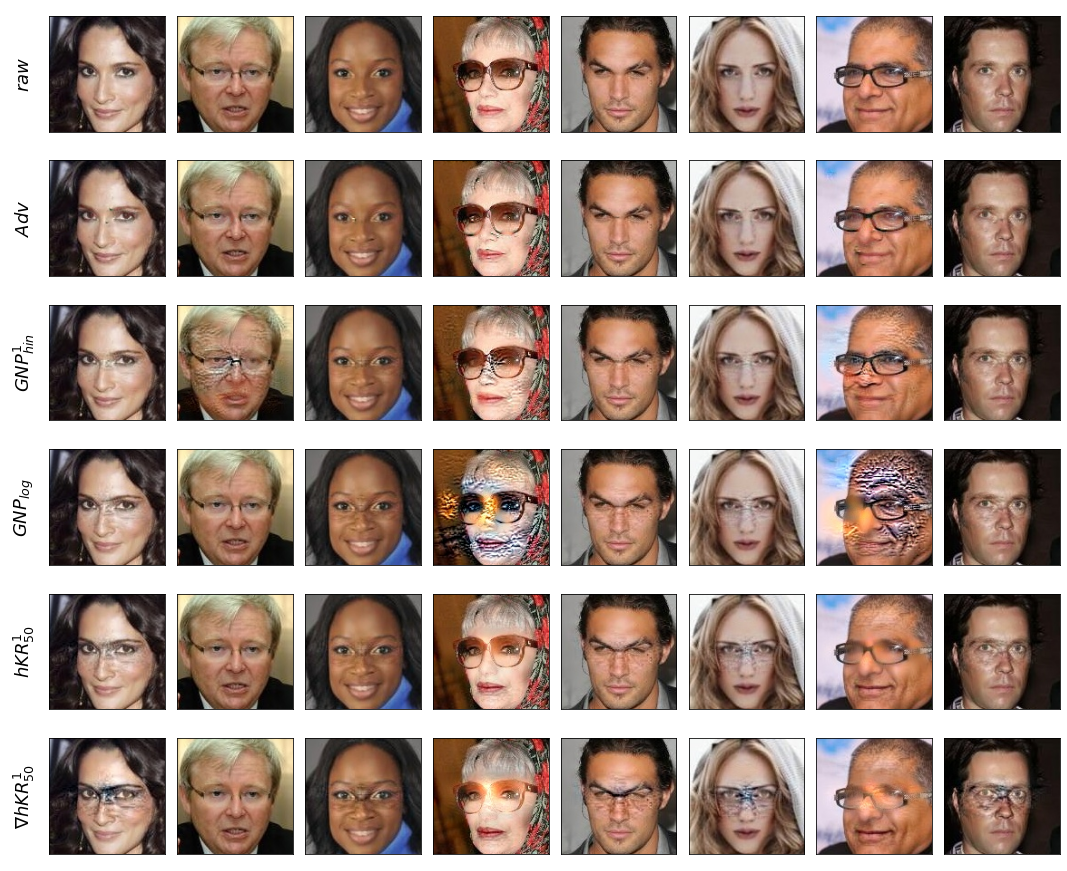
\includegraphics[width=1\linewidth]{cvpr_img/adversaries.png}

\caption{Adversarial examples on CelebA dataset. The first row is the input image.}
%Classical networks (1st line) and 1-lipschitz networks learned with binary crossentropy (2nd line) lead to invisble noise, whereas proposed solution (3rd line) add or remove dark pixels around the nasolabial fold}
\label{fig:Deep_fool_CelebA}
\end{figure*}


\section{Conclusion and future works}
\label{sec:conclusion}
This paper presents a novel classification framework and the associated deep learning process. Besides the interpretation of the classification task as a regularized optimal transport problem, we demonstrate that this new formalization has some valuable properties about error bounds and structural robustness regarding adversarial attacks. We also propose a systematic approach to ensure the 1-Lipschitz constraint of a neural network. This includes a state-of-the-art regularization algorithm and more precise constant evaluation for convolutional and pooling layers. Even if this regularization process can increase the computation time during learning, it doesn't impact inference. We developed an open source python library based on tensorflow for 1-Lipshitz layers and gradient preserving activation and pooling functions. This makes the approach very easy to implement and to use. \\

The experiment emphasizes the theoretical results and confirms that the classifier has good and predictable robustness to adversarial attacks with an acceptable cost on accuracy. We also show that our classifier forces adversarial attacks to explicitly modify the input. This suggest that our models can use adversarial attacks for explaining a prediction as it is done with counterfactual explanation in logic~\cite{DBLP:journals/corr/abs-1711-00399}.

In conclusion, we believe that this classification framework based on optimal transport is of great interest for critical problems since it provides both empirical and theoretical guarantees. %Future works will focus on the multiclass counterpart of the approach and on its applicability to large and deep networks.


\bibliographystyle{plain}
\bibliography{biblio} 
\newpage
\input{cvpr_parts/appendix_cvpr}
\end{document}